
% ===========================
\chapter{Grundlagen}
\label{grundlagen}
% ===========================

In diesem Kapitel werden die zum Verständnis nötigen Grundlagen für diese Arbeit erklärt. Dabei wird im Abschnitt \ref{grundlagen_fahren} der Stand der Technik von automatisierten Fahrfunktionen und deren Entwicklung beschrieben. Im Abschnitt \ref{grundlagen_nn} wird maschinelles Lernen im Allgemeinen und im Speziellen künstliche neuronale Netze, die für die Umsetzung dieser Arbeit nötig sind, beschrieben.


% ===========================
\section{Hochautomatisiertes Fahren}
\label{grundlagen_fahren}
% ===========================

Hochautomatisiertes Fahren wird in den vergangenen Jahren zunehmend von der Automobilindustrie vorangetrieben. Aktuelle \ac{FAS} wie der Spurhalteassistant oder die Abstandsregelung sind nach der Norm SAE J3016 (Abbildung \ref{fig_level_autonomes_fahren}) bei Level 2 des autonomen Fahrens eingeordnet. Mit neuen Technologien werden immer mehr Funktionen für automatisiertes Fahren entwickelt und verknüpft. Es entstehen zunehmend komplexe Fahrfunktionen mit einer steigenden Anzahl möglicher Fahrsituationen und Szenarien \cite{king2017identification}. Das stellt Automobilhersteller und Automobilzulieferer vor eine große Herausforderung, da die Systemkomplexität wächst. Das schließt sowohl die Entwicklung von \ac{FAS} als auch die dazu benötigten Testszenarien ein \cite{pfeffer2016continuous}.

In den folgenden Abschnitten wird erläutert wie aktuell diesen Herausforderungen begegnet wird. In Abschnitt \ref{grundlagen_fahren_entwicklung} wird ein allgemeiner Überblick über die aktuellen Entwicklungsmethodiken für \ac{FAS} gegeben. Danach werden in Abschnitt \ref{grundlagen_fahren_szenarien} bisherige Ansätze für die Klassifizierung von Fahrszenarien vorgestellt.

\begin{figure}[h]
\centering
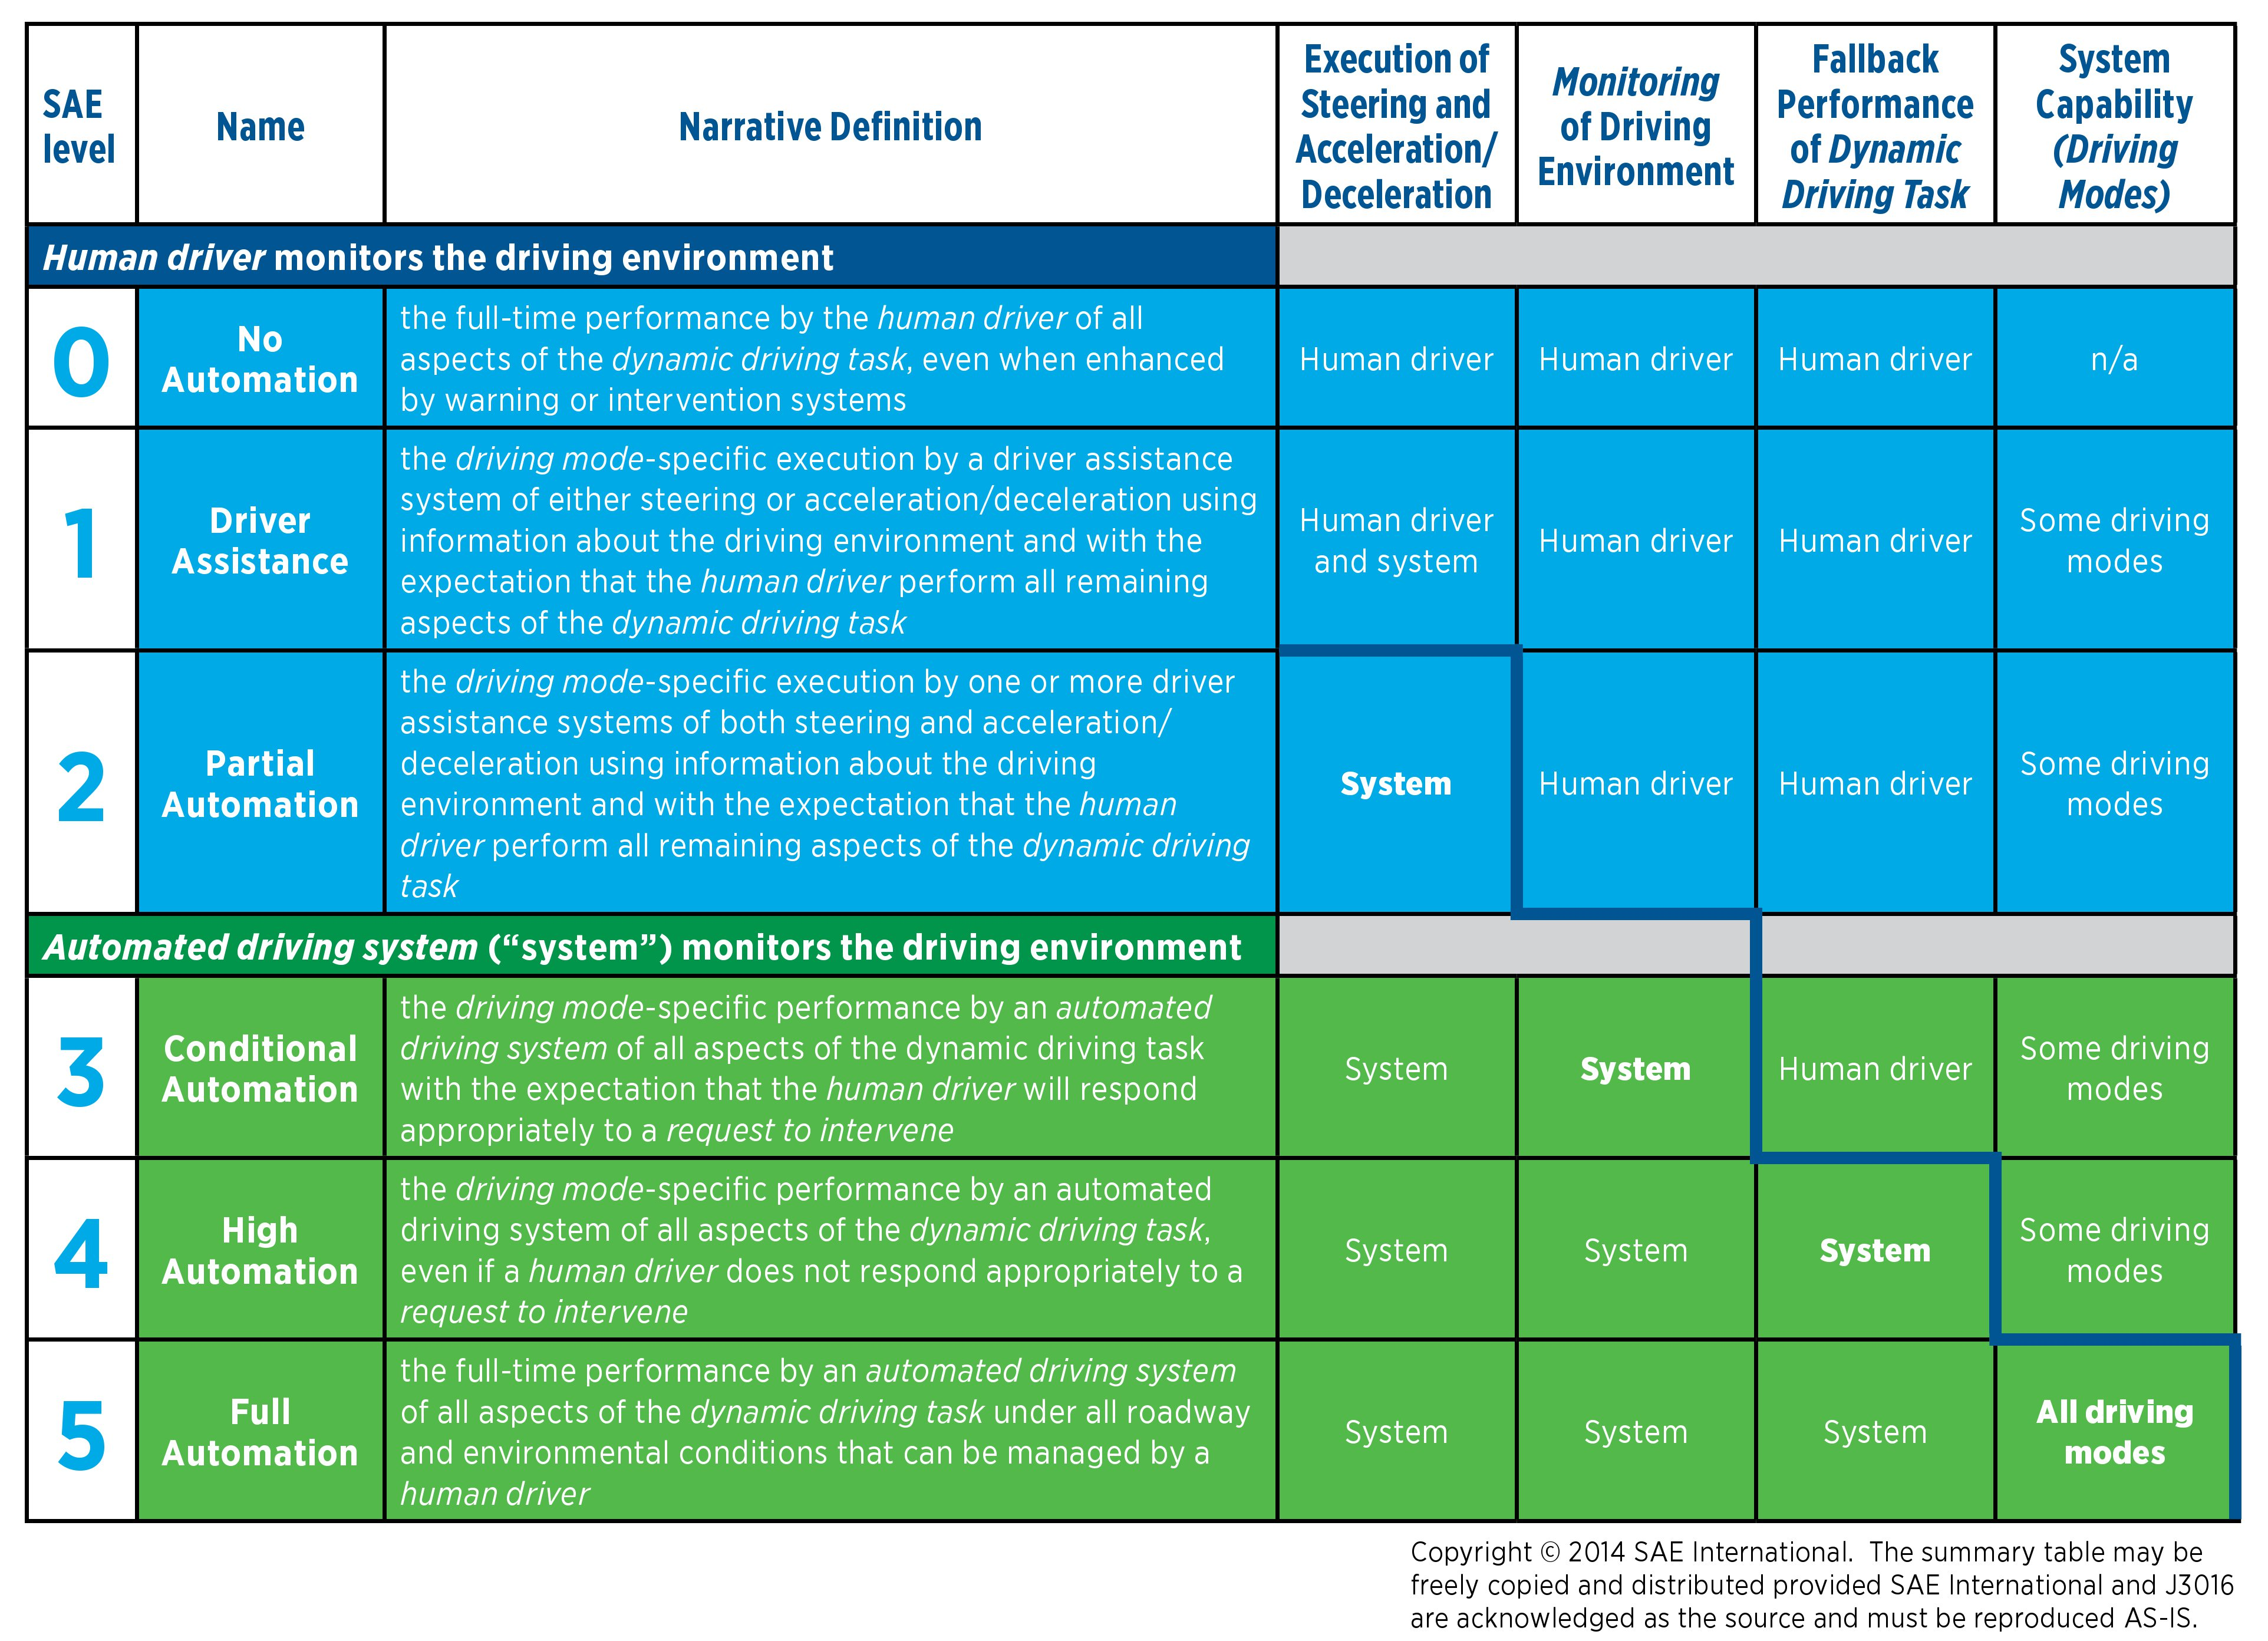
\includegraphics[scale=0.7]{level_autonomes_fahren.jpg}
\caption{Norm SAE J3016 für die Level des autonomen Fahrens \cite{sae2014taxonomy}}
\label{fig_level_autonomes_fahren}
\end{figure}


% ===========================
\subsection{Entwicklung von Fahrerassistenzfunktionen}
\label{grundlagen_fahren_entwicklung}
% ===========================

\ac{FAS} sind Funktionen im Kraftfahrzeug, die den Fahrer unterstützen. Diese Systeme nutzen Sensordaten, wie Radar-, Ultraschall-, oder Kameradaten, aus dem Fahrzeug um den Fahrer dann auf Basis der abgeleiteten Informationen zu unterstützen. Beispielsweise erkennt ein Spurhalteassistent wenn das Fahrzeug die Spur verlässt und kann die Fahrlinie korrigieren. 

\ac{FAS} werden in der Automobilindustrie mit dem V-Modell entwickelt. Das V-Modell ist ein chronologischer Entwicklungsprozess und aus der Softwareentwicklung adaptiert \cite{vmodell2005}. Das V-Modell kann in einen linken absteigenden und einen rechten aufsteigenden Ast unterteilt werden. Der linke Ast enthält die Funktionsanforderungen, die nach unten weiter detailliert und aufgeschlüsselt werden. Der rechte Ast umfasst aufsteigend Funktionstests auf dem jeweiligen Detaillierungsgrad \cite{hakuli2015virtuelle}. Das V-Modell ist in einer einfachen Version in Abbildung \ref{fig_v_modell} dargestellt.

\begin{figure}[h]
\centering
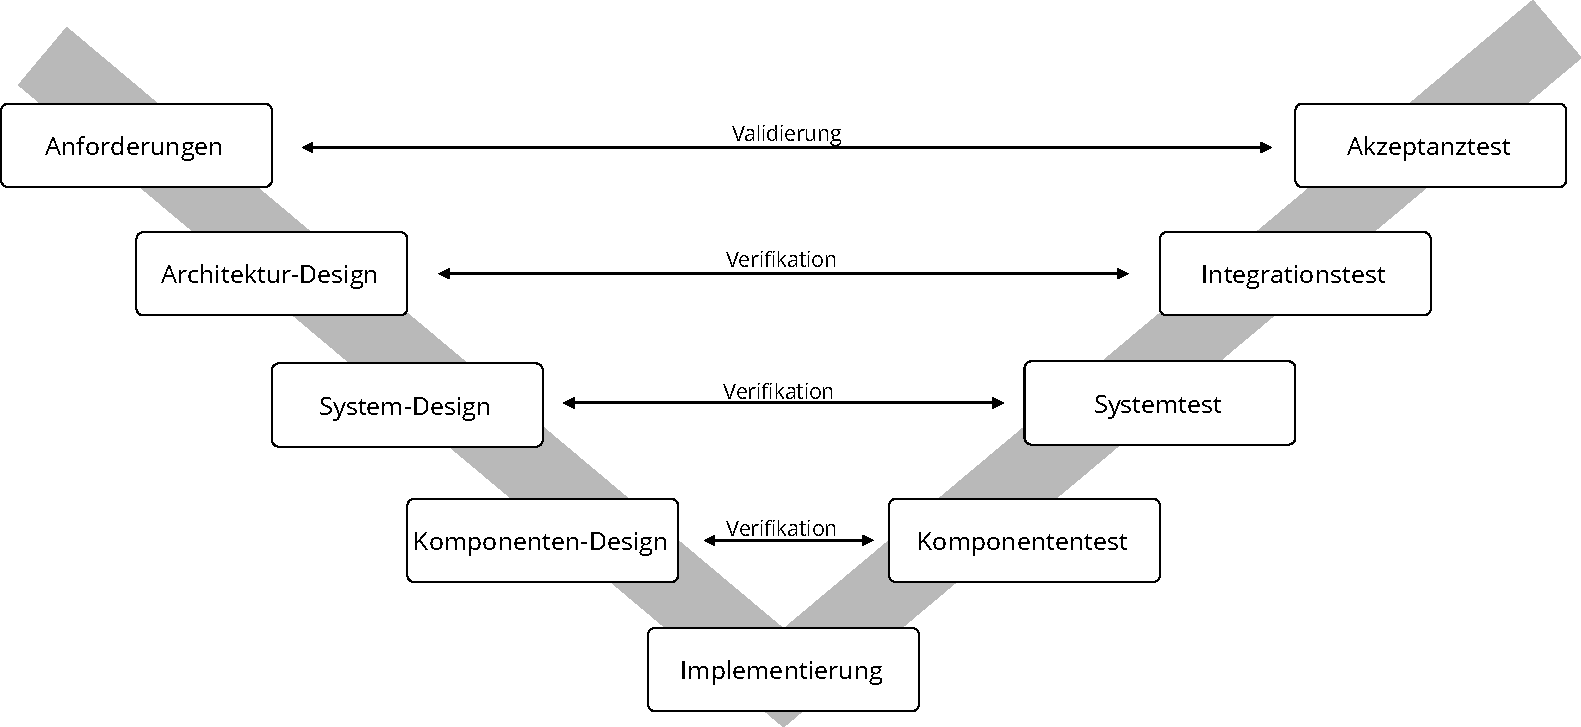
\includegraphics[scale=0.5]{v_modell.pdf}
\caption{V-Modell \cite{hakuli2015virtuelle}}
\label{fig_v_modell}
\end{figure}

Die Schritte auf dem absteigenden und aufsteigenden Ast haben jeweils eine Beziehung. Jeder Test auf dem aufsteigenden Ast verifiziert bzw. validiert den dazugehörigen Entwicklungsschritt auf dem absteigenden Ast. Demenstsprechend werden oben im V-Modell die Kundenanforderungen auf dem absteigenden Ast erfasst und auf dem aufsteigenden Ast validiert. Unten im V-Modell werden einzelne Hardware- oder Softwarekomponenten entwickelt, die die entsprechenden Kundenanforderungen von oben lösen sollen, und auf dem aufsteigenden Ast verifiziert \cite{hakuli2015virtuelle}.


% ===========================
\subsubsection{Testfälle für die Validierung und Verifikation}
% ===========================

Die Validierung und Verifikation von \ac{FAS} folgt dem Testkonzept. Ein Testkonzept umfasst die Analyse des Testobjektes, die Generierung von Testfällen, die Durchführung von Tests und schließlich die Testauswertung \cite{schuldt2013effiziente}. Diese Schritte sind der Abbildung \ref{fig_testfallerstellung} abgebildet.

\begin{figure}[h]
\centering
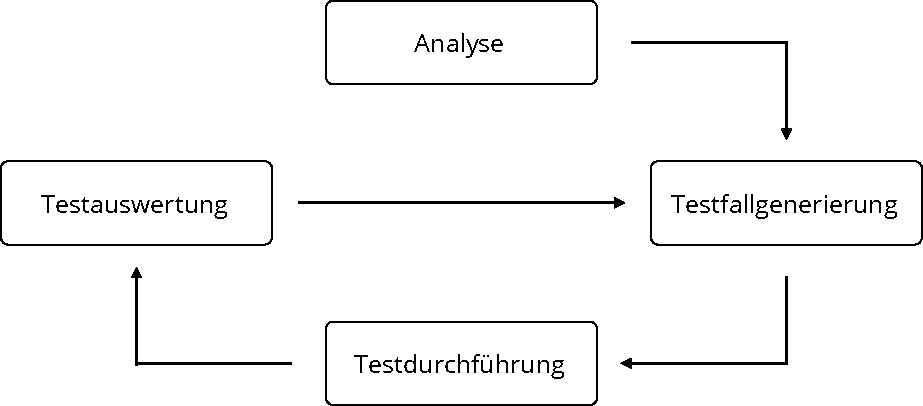
\includegraphics[scale=0.7]{testfallerstellung.pdf}
\caption{Schritte zur Testfallerstellung \cite{schuldt2013effiziente}}
\label{fig_testfallerstellung}
\end{figure}

Testfälle werden bereits möglichst früh im Entwicklungsprozess erstellt um die Qualität von \ac{FAS} und einzelnen Komponenten möglichst hoch zu halten \cite{wachenfeld2015freigabe}. Hierfür werden in der Praxis virtuelle Fahrversuche eingesetzt. Die Idee ist eine stufenweise Digitalisierung von Komponenten aus dem realen Fahrversuch mit den Zielen die Reproduzierbarkeit zu steigern, den Aufwand zu reduzieren und insgesamt flexibler zu werden. Im virtuellen Fahrversuch werden in der frühen Konzeptphase alle Komponenten virtuell getestet und dann schrittweise durch Hardwarekomponenten ersetzt. Schließlich werden alle Komponenten im realen Fahrversuch auf der Straße mit einem realem Fahrer und anderen Verkehrsteilnehmern getestet \cite{hakuli2015virtuelle}.

Beim virtuellen Fahrversuch spielen die Konzepte \ac{MiL}, \ac{SiL}, \ac{HiL} und \ac{ViL} eine wichtige Rolle. Mit \ac{MiL} und \ac{SiL} werden Funktionen auf Basis von Simulationsmodellen getestet \cite{berg2015vehicle}, indem Hardwarekomponenten simuliert werden. Mit fortschreitender Entwicklung werden immer mehr Simulationskomponenten durch die entsprechende Hardware ersetzt und mit \ac{HiL} getestet \cite{hakuli2015virtuelle}. \ac{ViL} schließt schließlich die Lücke zwischen virtuellem Fahrversuch und realem Fahrversuch. Dieses Testkonzept macht die Komplexität bei der Entwicklung von \ac{FAS} beherrschbar und reduziert den Testaufwand \cite{schwab2014durchgangige}. Für die Freigabe von \ac{FAS} ist die Realfahrt die wichtigste Methode, da sie aktuell die beste Validierung bei annehmbaren ökonomischen Aufwand ist \cite{wachenfeld2015freigabe}.

Mit steigender Automatisierung von \ac{FAS} steigt auch die Anzahl möglicher Situationen in denen die Funktionen ohne Fahrer ablaufen müssen. Um alle Funktionen ausreichend testen zu können, steigt die Anzahl der benötigten Testfälle. Testfälle müssen alle potentiell möglichen Situationen, in denen das \ac{FAS} zum Einsatz kommen kann, abdecken. Dadurch steigt mit hochautomatisierten Funktionen der Aufwand für Validierung und Verifikation mit Testfällen \cite{bach2017reactive}. Eine Möglichkeit für die Reduzierung von Testfällen ist es kritische Situationen zu finden und Testfälle mit weniger kritischen Situationen zu entfernen \cite{wachenfeld2015freigabe}.

Heute werden Testfälle auf der Basis von Szenarienkatalogen abgeleitet \cite{putz2017system}. Diese Kataloge enthalten alle bekannten Szenarien in denen sich ein Fahrzeug befinden kann. Sie sind jedoch vor dem Hintergrund erstellt worden, dass zu jeder Zeit ein Fahrer das Kraftfahrzeug überwacht und steuert \cite{wachenfeld2015freigabe}. Bei neuen hochautomatisierten \ac{FAS} für Stufe 3 und 4 des autonomen Fahrens, ist dies nicht mehr gegeben. Die Sicherheit des Gesamtsystems muss in breiterem Spektrum mit einer Vielzahl hochkomplexer Szenarien ohne Eingriff des Fahrers garantiert werden können.

Für die Erstellung von Testfällen müssen daher alle potentiell möglichen kritischen Szenarien bekannt sein. Der Ansatz in dieser Arbeit ist es bekannte Szenarien zu klassifizieren und auf diese Weise bisher unbekannte und möglicherweise kritische Szenarien zu finden. Dies soll mit Hilfe von simulierten Daten geschehen, um die Skalierbarkeit mit angemessenem Aufwand garantieren zu können. Das Konzept hierzu wird im Detail in Kapitel \ref{konzept} vorgestellt.

 Im nächsten Abschnitt werden andere Arbeiten, die die Klassifizierung von Szenarien untersucht haben, vorgestellt und wichtige Grundbegriffe definiert.


% ===========================
\subsection{Klassifizierung von Szenarien}
\label{grundlagen_fahren_szenarien}
% ===========================

In diesem Abschnitt werden zu Beginn die Terminologien von Szene, Situation und Szenario unterschieden und definiert. Im Anschluss wird auf bisherige Arbeiten zur Szenarienerkennung eingegangen.

In dieser Arbeit werden Szene, Situation und Szenario nach Ulbrich et al. \cite{ulbrich2015defining} definiert. In Abbildung \ref{fig_relation_sc_sc} wird die Beziehung zwischen Szene und Szenario dargestellt.

\noindent\textbf{Szene}\\
Eine Szene ist eine Momentaufnahme von der Umgebung einschließlich der räumlichen Szenerie,  allen dynamischen Elementen, der Selbstdarstellung aller Akteure und Beobachter, sowie die Beziehung zwischen diesen Entitäten. Nur in einer Simulation kann eine Szene vollständig und allumFASsend beobachtet und erfasst werden (Ground Truth). In der realen Welt dagegen, ist die Beschreibung einer Szene immer unvollständig, fehlerhaft, unsicher und subjektiv von einem oder mehreren Beobachtern.

\noindent\textbf{Situation}\\
Eine Situation ist die Gesamtheit aller Umstände, die für die Auswahl einer angemessenen Entscheidung zu einem bestimmten Zeitpunkt berücksichtigt werden müssen. Sie umfasst alle relevanten Zustände, Möglichkeiten und Einflussgrößen für ein Verhalten. Eine Situation wird abgeleitet von einer Szene durch die Auswahl von Informationen basierend auf kurzzeitigen sowie langfristigen Zielen und Werten. Eine Situation ist daher per Definition immer subjektiv von einem Beobachter.

\noindent\textbf{Szenario}\\
Ein Szenario besteht aus mehrerer aufeinander folgenden Szenen und beschreibt diese zeitliche Entwicklung. Handlungen, Ereignisse, Ziele und Werte können für eine Charakterisierung der zeitlichen Entwicklung eines Szenarios spezifiziert werden. Anders als eine Szene, umfasst ein Szenario einen definierten Zeitraum.

\begin{figure}[h]
\centering
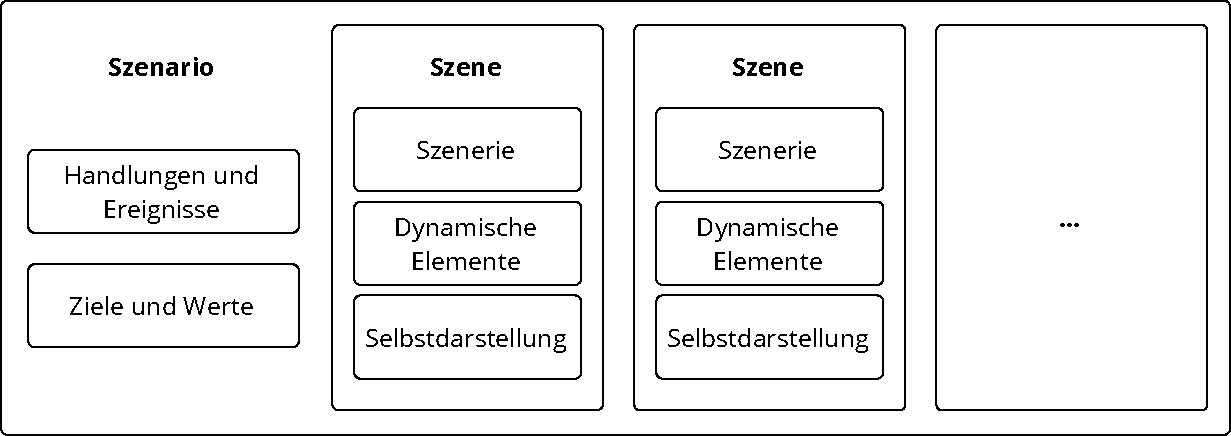
\includegraphics[scale=0.7]{relation_sc_sc.pdf}
\caption{Zusammenhang zwischen Szene und Szenario \cite{ulbrich2015defining}}
\label{fig_relation_sc_sc}
\end{figure}

Neben den Begriffen Szene, Situation und Szenario wird auch oft der Begriff Manöver verwendet. Bach et al. \cite{bach2016model} definieren ein Manöver als einen Status innerhalb eines Szenarios. Dabei sind Situation jeweils Übergangsbedingungen zwischen einzelnen Manövern. So setzt sich beispielsweise das Szenario \textit{Überholen} aus den Manövern \textit{Spurwechsel nach links}, \textit{Beschleunigung}, \textit{Spurwechsel nach rechts} und \textit{Bremsvorgang} zusammen. Zwischen den einzelnen Manövern gibt es Situation wie \textit{langsameres Auto voraus} oder \textit{langsameres Auto links überholt}, die jeweils ein neues Manöver einleiten.

Je nachdem wie granular Szenarien bzw. wie grob Manöver definiert werden, können Szenarien und Manöver nicht klar voneinander abgegrenzt werden. So kann ein einzelnes Manöver auch bereits ein gesamtes Szenario darstellen. Zum Beispiel kann das Manöver \textit{Spurwechsel} bereits als Szenario definiert werden. Aus diesem Grund wird in dieser Arbeit im Folgenden ausschließlich von Szenarios gesprochen.

Da sich diese Arbeit größtenteils auf die Klassifizierung von Szenarien fokussiert, wird in den folgenden Absätzen eine erweiterte Definition von Szenarien nach Bagschik et al. \cite{bagschik2017szenarien} gegeben. Diese Definition unterteilt den Begriff in drei weitere Abstraktionsebenen: Funktionale, logische und konkrete Szenarien.

Funktionale Szenarien sind auf der semantischen Ebene formuliert. Entitäten und Beziehungen werden widerspruchsfrei in sprachlichen Texten beschrieben. Dabei ist das Vokabular klar definiert und wird eindeutig für alle zu beschreibenden Szenarien verwendet. Je nachdem wie detailliert ein Szenario beschrieben werden soll, muss ein geeignetes Vokabular definiert werden. Funktionale Szenarien können in einzelne oder mehrere logische Szenarien überführt werden.

Logische Szenarien sind detaillierter als funktionale Szenarien, indem  Entitäten und Beziehung in quantitive Parameterbereiche übersetzt werden. Parameterbereiche können dabei mit statistischen Verteilungen (Normalverteilung, Gleichverteilung etc.) modelliert werden. Zusätzlich können Beziehungen zwischen Entitäten mit numerischen Bedingungen (e.g. Fahrzeug A muss auf derselben Spur fahren wie Fahrzeug B) oder Korrelationsfunktionen (e.g. Abstand zwischen Fahrzeug A und Fahrzeug B in Abhängigkeit der Geschwindigkeit) ausgedrückt werden.

Konkrete Szenarien haben den höchsten Detailgrad und Entitäten und Beziehungen werden mit festen Parametern definiert. Logische Szenarien können in einzelne oder mehrere konkrete Szenarien überführt werden.

Ein Beispiel zu jeder Abstraktionsebene (funktional, logisch, konkret) ist in Abbildung \ref{fig_funktional_logisch_konrekt} gegeben.

\begin{figure}[h]
\centering
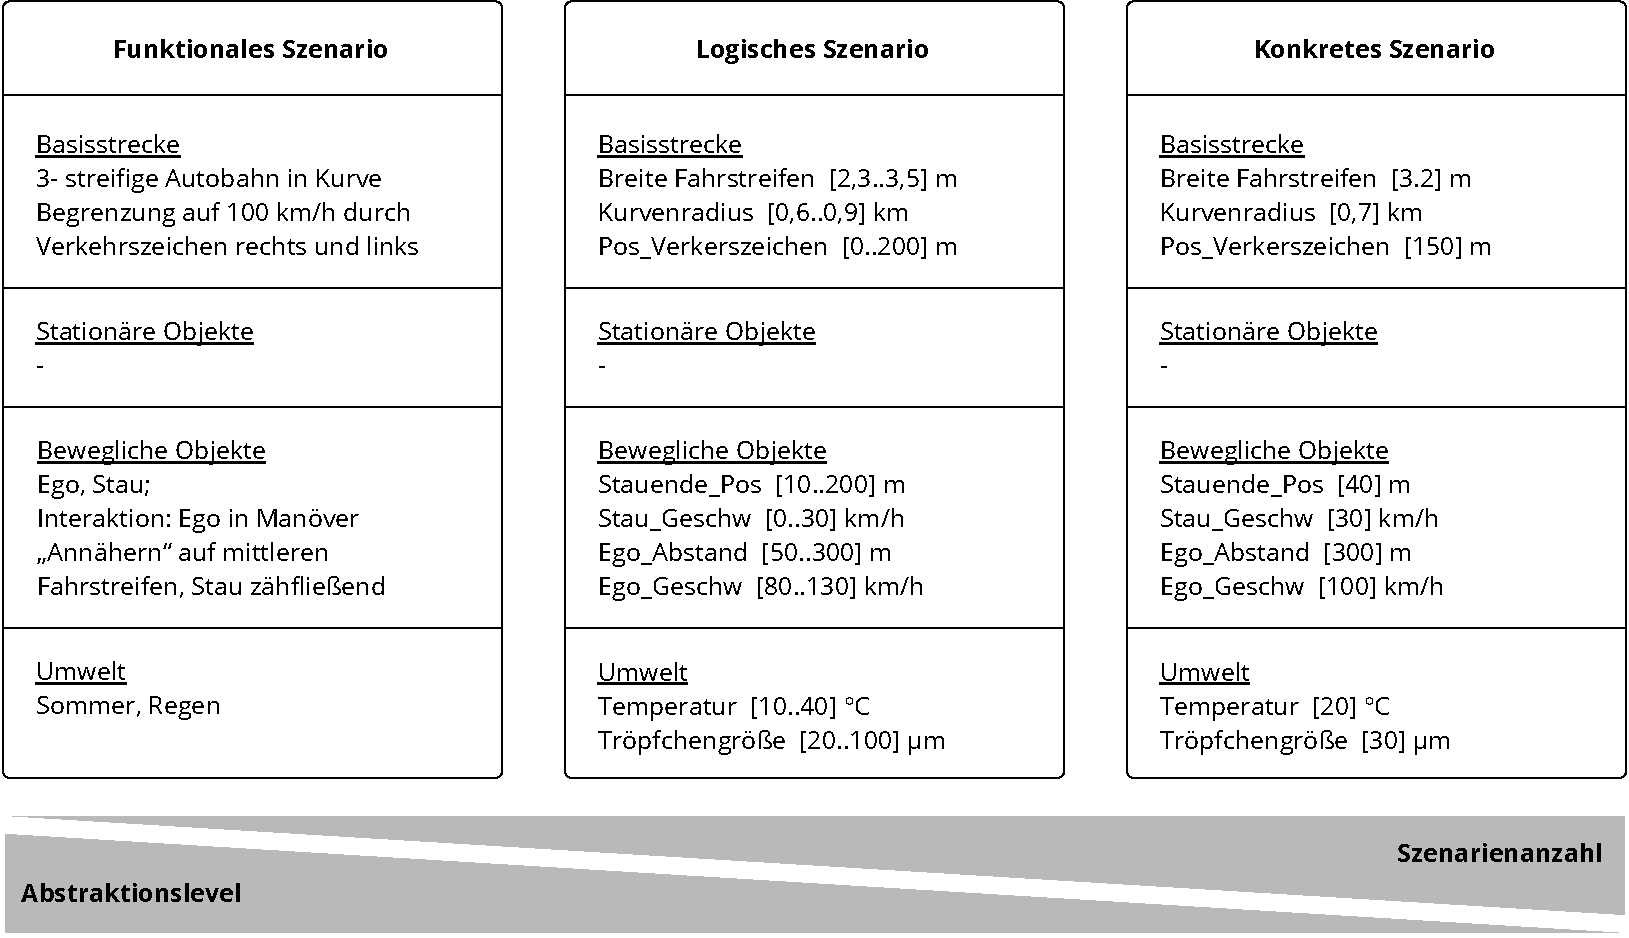
\includegraphics[scale=0.5]{funktional_logisch_konrekt.pdf}
\caption{Beispiel für ein funktionales, logisches und konkretes Szenario \cite{bagschik2017szenarien}}
\label{fig_funktional_logisch_konrekt}
\end{figure}


% ===========================
\subsubsection{Klassifizierung von Fahrszenarien}
% ===========================

Wie in Abschnitt \ref{grundlagen_fahren_entwicklung} beschrieben ist die Klassifizierung von Szenarien ein wichtiges Element für die Erstellung von Testfällen und die Sicherung von \ac{FAS}. In den vergangenen Jahren wurden bereits einige Methoden zur Klassifizierung von Szenarien veröffentlicht. In den folgenden Absätzen werden die relevanten Arbeiten (Anzahl 12) seit 2014 kurz vorgestellt.

Für die Klassifizierung wurden verschiedene Sensordaten aus dem Fahrzeug verwendet. Die Autoren von fünf Arbeiten haben ein Smartphone im Fahrzeug platziert und Beschleunigungs-, Gyroskop-, GPS- und Magnetometer-Daten für die Klassifizierung ausgelesen und verwendet \cite{xie2018driving, cervantes2016vehicle, woo2016manoeuvre, camlica2016feature, arroyo2016adaptive}. Die Verwendung von Smartphone-Daten wurde mit der einfachen und kostengünstigen Umsetzung begründet. Vier andere Arbeiten verwendeten Sensordaten wie \textit{Lenkwinkel}, \textit{Fahrzeuggeschwindigkeit}, \textit{laterale Geschwindigkeit}, \textit{Giergeschwindigkeit} und die \textit{Position des Gas- und Bremspedals}, die sie aus dem CAN-Bus des Fahrzeugs ausgelesen haben \cite{zheng2017lane, zheng2015non, li2015lane, zheng2014threshold}. Drei weitere Arbeiten basierten ihre Experimente auf Daten aus einem Fahrsimulator \cite{sun2017robust, zheng2016drivers} und realen Testfahrten \cite{gruner2017spatiotemporal}. Die verwendeten Daten waren der \textit{laterale Abstand zwischen Fahrzeug und Fahrbahnmarkierung}, \textit{Spurabfahrtsbetrag}, \textit{Beschleunigung}, \textit{Lenkwinkel}, \textit{Lenkgeschwindigkeit}, \textit{Lenkmoment} und \textit{Ort}, \textit{Ausrichtung}, und \textit{Geschwindigkeit} des Ego-Fahrzeugs und benachbarten Objekten. Dabei wurde nicht weiter spezifiziert wie die Daten ausgelesen wurden.

Auf Basis der Sensordaten wurden verschiedene Klassifikatoren erstellt. Es wurden die Methoden \ac{SVM} \cite{sun2017robust, cervantes2016vehicle, woo2016manoeuvre, camlica2016feature, zheng2016drivers, zheng2015non}, \ac{RF} \cite{xie2018driving, cervantes2016vehicle, zheng2016drivers}, \ac{kNN} \cite{zheng2017lane, camlica2016feature, zheng2016drivers}, \ac{HMM} \cite{zheng2017lane, li2015lane}, \ac{FRC} \cite{cervantes2016vehicle, arroyo2016adaptive}, Bayesian Inference Model \cite{sun2017robust}, \ac{CNN} \cite{gruner2017spatiotemporal}, Decision Tree \cite{zheng2014threshold} und Naive Bayes \cite{camlica2016feature} verwendet. Da es für diese Arbeit nicht relevant ist, werden die Methoden an dieser Stelle nicht im Detail erläutert, es wird lediglich auf die jeweiligen Quellen verwiesen.

In Tabelle \ref{tab_szenarienerkennung} sind alle Arbeiten zusammengefasst. Neben den verwendeten Methoden zur Klassifizierung sind die jeweils verwendeten Sensordaten und die klassifizierten Szenarien aufgeführt.

\small
\begin{longtable}[c]{p{1,5cm} p{4cm} p{2,5cm} p{4cm}}
\textbf{Quelle} & \textbf{Sensordaten} & \textbf{Klassifikator} & \textbf{Szenarien} \\
\hline
\endhead

\cite{xie2018driving} & Beschleunigung, Gyroskop und GPS von einem Smartphone das im Fahrzeug platziert ist & \ac{RF} & Abbiegen, links abbiegen, rechts abbiegen, beschleunigen, bremsen, stoppen, Spurwechsel nach links, Spurwechsel nach rechts \\
\hline

\cite{zheng2017lane} & Lenkwinkel und Fahrzeuggeschwindwigkeit aus dem CAN-Bus & \ac{kNN}, \ac{HMM} & Spurwechsel nach links, Spurwechsel nach rechts, Spur halten \\
\hline

\cite{sun2017robust} & Lateraler Abstand zwischen Fahrzeug und Fahrbahnmarkierung von einem Fahrsimulator & \ac{SVM}, Bayesian Inference Model & Spurwechsel nach links, Spurwechsel nach rechts, Spur halten \\
\hline

\cite{gruner2017spatiotemporal} & Ort, Ausrichtung und Geschwindigkeit des Ego-Fahrzeugs und benachbarten Objekten von realen Testfahrten & \ac{CNN} auf Basis von gestapelten Positionsgittern der Objekte & Frei fahren, anderes Fahrzeug voraus, anderes Fahrzeug überholt Ego-Fahrzeug, Querverkehr vor Ego-Fahrzeug \\
\hline

\cite{cervantes2016vehicle} & Beschleunigung von einem Smartphone das im Fahrzeug platziert ist & \ac{RF}, \ac{SVM}, \ac{FRC} & Einparken, geparkt, frei fahren, stoppen \\
\hline

\cite{woo2016manoeuvre} & Beschleunigung, Gyroskop, GPS und Magnetometer von einem Smartphone das im Fahrzeug platziert ist & \ac{SVM} & Stoppen, beschleunigen, bremsen, links abbiegen, rechts abbiegen \\
\hline

\cite{camlica2016feature} & Beschleunigung, Gyroskop und GPS von einem Smartphone das im Fahrzeug platziert ist & \ac{SVM}, \ac{kNN}, Naive-Bayes & Stoppen, beschleunigen, frei fahren, bremsen, Spurwechsel nach links, Spurwechsel nach rechts, links abbiegen, rechts abbiegen, in Kreisverkehr eintreten, aus Kreisverkehr austreten \\
\hline

\cite{zheng2016drivers} & Spurabfahrtsbetrag, Beschleunigung, Lenkwinkel, Lenkgeschwindigkeit und Lenkmoment von einem Fahrsimulator & \ac{SVM}, \ac{kNN}, \ac{RF} & Spurwechsel nach links, Spurwechsel nach rechts, Spur halten \\
\hline

\cite{arroyo2016adaptive} & Beschleunigung, Gyroskop und GPS von einem Smartphone das im Fahrzeug platziert ist & \ac{FRC} & Lenken, beschleunigen, bremsen, Bodenwelle \\
\hline

\cite{zheng2015non} & Fahrzeuggeschwindigkeit und Lenkwinkel aus dem CAN-Bus & \ac{SVM} & links abbiegen, rechts abbiegen, Spurwechsel nach links, Spurwechsel nach rechts, Kurve nach links, Kurve nach rechts, geradeaus fahren, stoppen \\
\hline

\cite{li2015lane} & Fahrzeuggeschwindigkeit, Position des Gas- und Bremspedals, Lenkwinkel, Laterale Beschleunigung und Giergeschwindigkeit aus dem CAN-Bus & \ac{HMM} & Spurwechsel nach links, Spurwechsel nach rechts, Spur halten \\
\hline

\cite{zheng2014threshold} & Fahrzeuggeschwindigkeit, Lenkwinkel, Drehzahl und Position des Gas- und Bremspedals aus dem CAN-Bus & Decision Tree auf Basis von Schwellenwerten & links abbiegen, rechts abbiegen, Spurwechsel nach links, Spurwechsel nach rechts, Kurve nach links, Kurve nach rechts, geradeaus fahren, stoppen \\

\hline
\caption{Bisherige Arbeiten zur Szenarienerkennung}
\label{tab_szenarienerkennung}
\end{longtable}
\normalsize

Die Datenerhebungen in den vergangenen Arbeiten wurde vor dem Hintergrund durchgeführt vordefinierte Szenarien zu erkennen. Von diesen Szenarien wurden die benötigten Sensordaten abgeleitet und dann mit bestimmten Methoden verschiedene Klassifikatoren erstellt. Bis auf in der Arbeit von Gruner \cite{gruner2017spatiotemporal} werden für die Klassifizierung von Fahrszenarien bisher keine \acp{DNN} verwendet. Und in seiner Arbeit verwendet er keine Kamerabildern, sondern mit gespapelten Matritzen, auf denen jeweils die Positionen aller Verkehrsteilnehmer markiert sind. Nach Grunder \cite{gruner2017spatiotemporal} wird sich die zukünftige Forschung mit tieferen Netzstrukturen wie \acp{RNN} beschäftigen, um zeitabhängige Szenarien noch besser zu verstehen.

 Mit den bisherigen Ansätzen können bekannte Szenarien gut klassifiziert werden. Unbekannte bzw. neue Szenarien werden allerdings nur sehr bedingt erkannt, weil die Datengrundlage für die bekannten Szenarien optimiert ist. Das bedeutet, dass Daten, die für die Erkennung von bisher unbekannten Szenarien möglicherweise relevant sind, nicht erfasst und daher nicht für die Erstellung des Klassifikators verwendet werden. 

Im Gegensatz zu den bisherigen Arbeiten, soll in dieser Arbeit die Verwendung von Kameradaten für die Klassifizierung von Szenarien untersucht werden. Als Klassifikator soll ein bild- und zeitsensitives \ac{DNN} verwendet werden. Damit sollen auch bisher unbekannte Einflüsse, die auf den Bildern zu sehen sind, für die Klassifizierung berücksichtigt werden. Der Ansatz wird im Detail in Kapitel \ref{konzept} erklärt.

% ===========================
\section{Künstliche Neuronale Netze}
\label{grundlagen_nn}
% ===========================

Dieses Kapitel gibt einen Überblick zu künstlichen neuronalen Netzen (nachfolgend neuronale Netze genannt) mit einem Schwerpunkt auf Bilderkennung mit \acp{CNN} und Sequenzerkennung mit \acp{LSTM}. Im folgenden Abschnitt \ref{grundlagen_nn_ml} werden neuronale Netze in den Gesamtkontext von maschinellem Lernen gestellt. Im Anschluss werden in Abschnitt \ref{grundlagen_nn_entwicklung} die Grundlagen zu neuronalen Netzen erläutert. Dann werden komplexe Architekturen von neuronalen Netzen zur Bilderkennung in Abschnitt \ref{grundlagen_nn_cnn} und zur Szequenzerkennung in Abschnitt \ref{grundlagen_nn_rnn} erklärt. In Abschnitt \ref{grundlagen_nn_synthetisch} wird auf das Training mit synthetischen Daten eingegangen und im letzten Abschnitt \ref{grundlagen_nn_video} wird die aktuelle Forschung zu Videoklassifizierung vorgestellt.

% ===========================
\subsection{Einordnung im maschinellen Lernen}
\label{grundlagen_nn_ml}
% ===========================

Maschinelles Lernen wird oft als ein Teil des Bereichs künstliche Intelligenz beschrieben. Dabei wird maschninelles Lernen nach Mitchell \cite{mitchell1997machine} wie folgt definiert:

\begin{quote}
\textit{\glqq Ein Computerprogramm lernt aus der Erfahrung E in Bezug auf eine Klasse von Aufgaben T und dem Leistungsmaß P, wenn seine Leistung, gemessen mit P, bei Aufgaben aus T sich mit Erfahrung E verbessert.\grqq}
\end{quote}

Da maschinelles Lernen sehr viele Bereiche umfasst, wird hier nur auf die relevanten Teile für diese Arbeit eingegangen und auf \cite{mitchell1997machine} verwiesen. Maschinelles Lernen kann in drei verschiedenen Kategorien eingeteilt werden. Diese werden in den folgenden Absätzen beschrieben.

Überwachtes Lernen (engl. supervised learning) beschreibt einen Lernprozess in dem die Trainingsdaten sowohl Inputvektoren als auch die zugehörigen Zielvektoren enthalten \cite{bishop2006pattern}. Ein Beispiel dafür ist ein Klassifizierungsproblem von Buchstaben bei dem sowohl die Bilder der einzelnen Buchststaben als auch deren zugehörige Klasse (abgebildeter Buchstabe) einem Trainingsalgorithmus übergeben werden. Neben Klassifizierungsproblemen fallen auch Regressionsprobleme in diese Kategorie.

Beim unüberwachten Lernen (engl. unsupervised learning) enhalten die Trainingsdaten ausschließlich die Inputvektoren, ohne die dazugehörigen Zielvektoren. Das Ziel dabei ist es Muster in den gegebenen Daten zu erkennen um beispielsweise Cluster zu bilden \cite{bishop2006pattern}. Das Clustering von Kundengruppen, die bisher unbekannt waren, fällt in diese Kategorie des maschinellen Lernens.

Das verstärkende Lernen (engl. reinforcement learning) ist eine Methodik in der der Trainingsalgorithmus mit Situationen konfrontiert wird und jeweils aus einer Reihe von gegebenen Handlungen wählen kann. Das Ziel dabei ist es das Endergebnis, das auf der Wahl aller Handlungen basiert, zu maximieren \cite{sutton1998introduction}. Ein Beispiel hierfür ist selbstständige Erlenen des Brettspiels Schach.


% ===========================
\subsubsection{Klassifizierung}
% ===========================

In dieser Arbeit wird ein Konzept für die Klassifizierung von Fahrszenarien - damit in der Kategorie überwachtes Lernen - entwickelt und umgesetzt. Das Ziel von Klassifizierungsalgorithmen ist es gegebene Objekte auf Basis ihrer Eigenschaften einer Klasse zuzuordnen. Dabei sollen die Objekte innerhalb einer Klasse eine möglicht geringe Varianz und zwischen verschiedenen Klassen eine möglichst hohe Varianz besitzen. Klassifizierungsalgorithmen arbeiten dafür mit Trainingsdaten, die aus Inputvektoren und Zielvektoren bestehen. Ein Inputvektor enthällt alle Eigenschaften und der Zielvektor die jeweilige Klasse des Objektes. In Abbildung \ref{fig_klassifizierung} ist beispielhaft ein Datensatz mit zwei Klassen dargestellt. Die Objekte im Datensatz haben jeweils die Eigenschaften $x_1$ und $x_2$.

\begin{figure}[h]
\centering
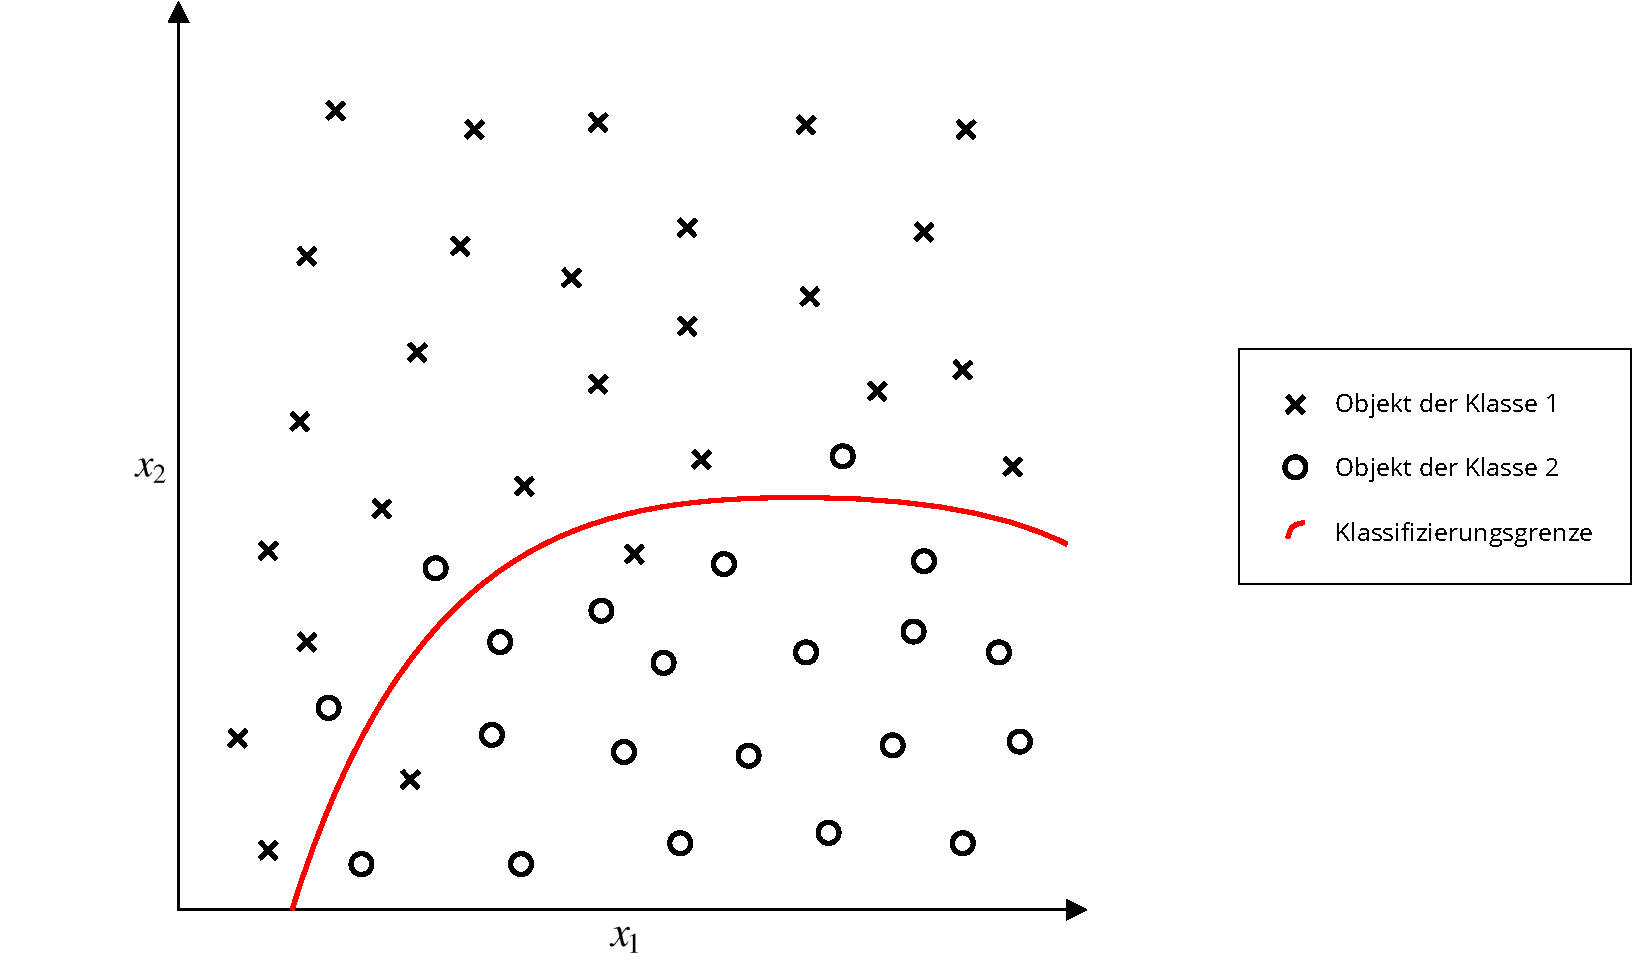
\includegraphics[scale=0.5]{klassifizierung.pdf}
\caption{Beispiel einer Klassifizierung mit zwei Klassen}
\label{fig_klassifizierung}
\end{figure}


Overfitting

\begin{figure}[h]
\centering
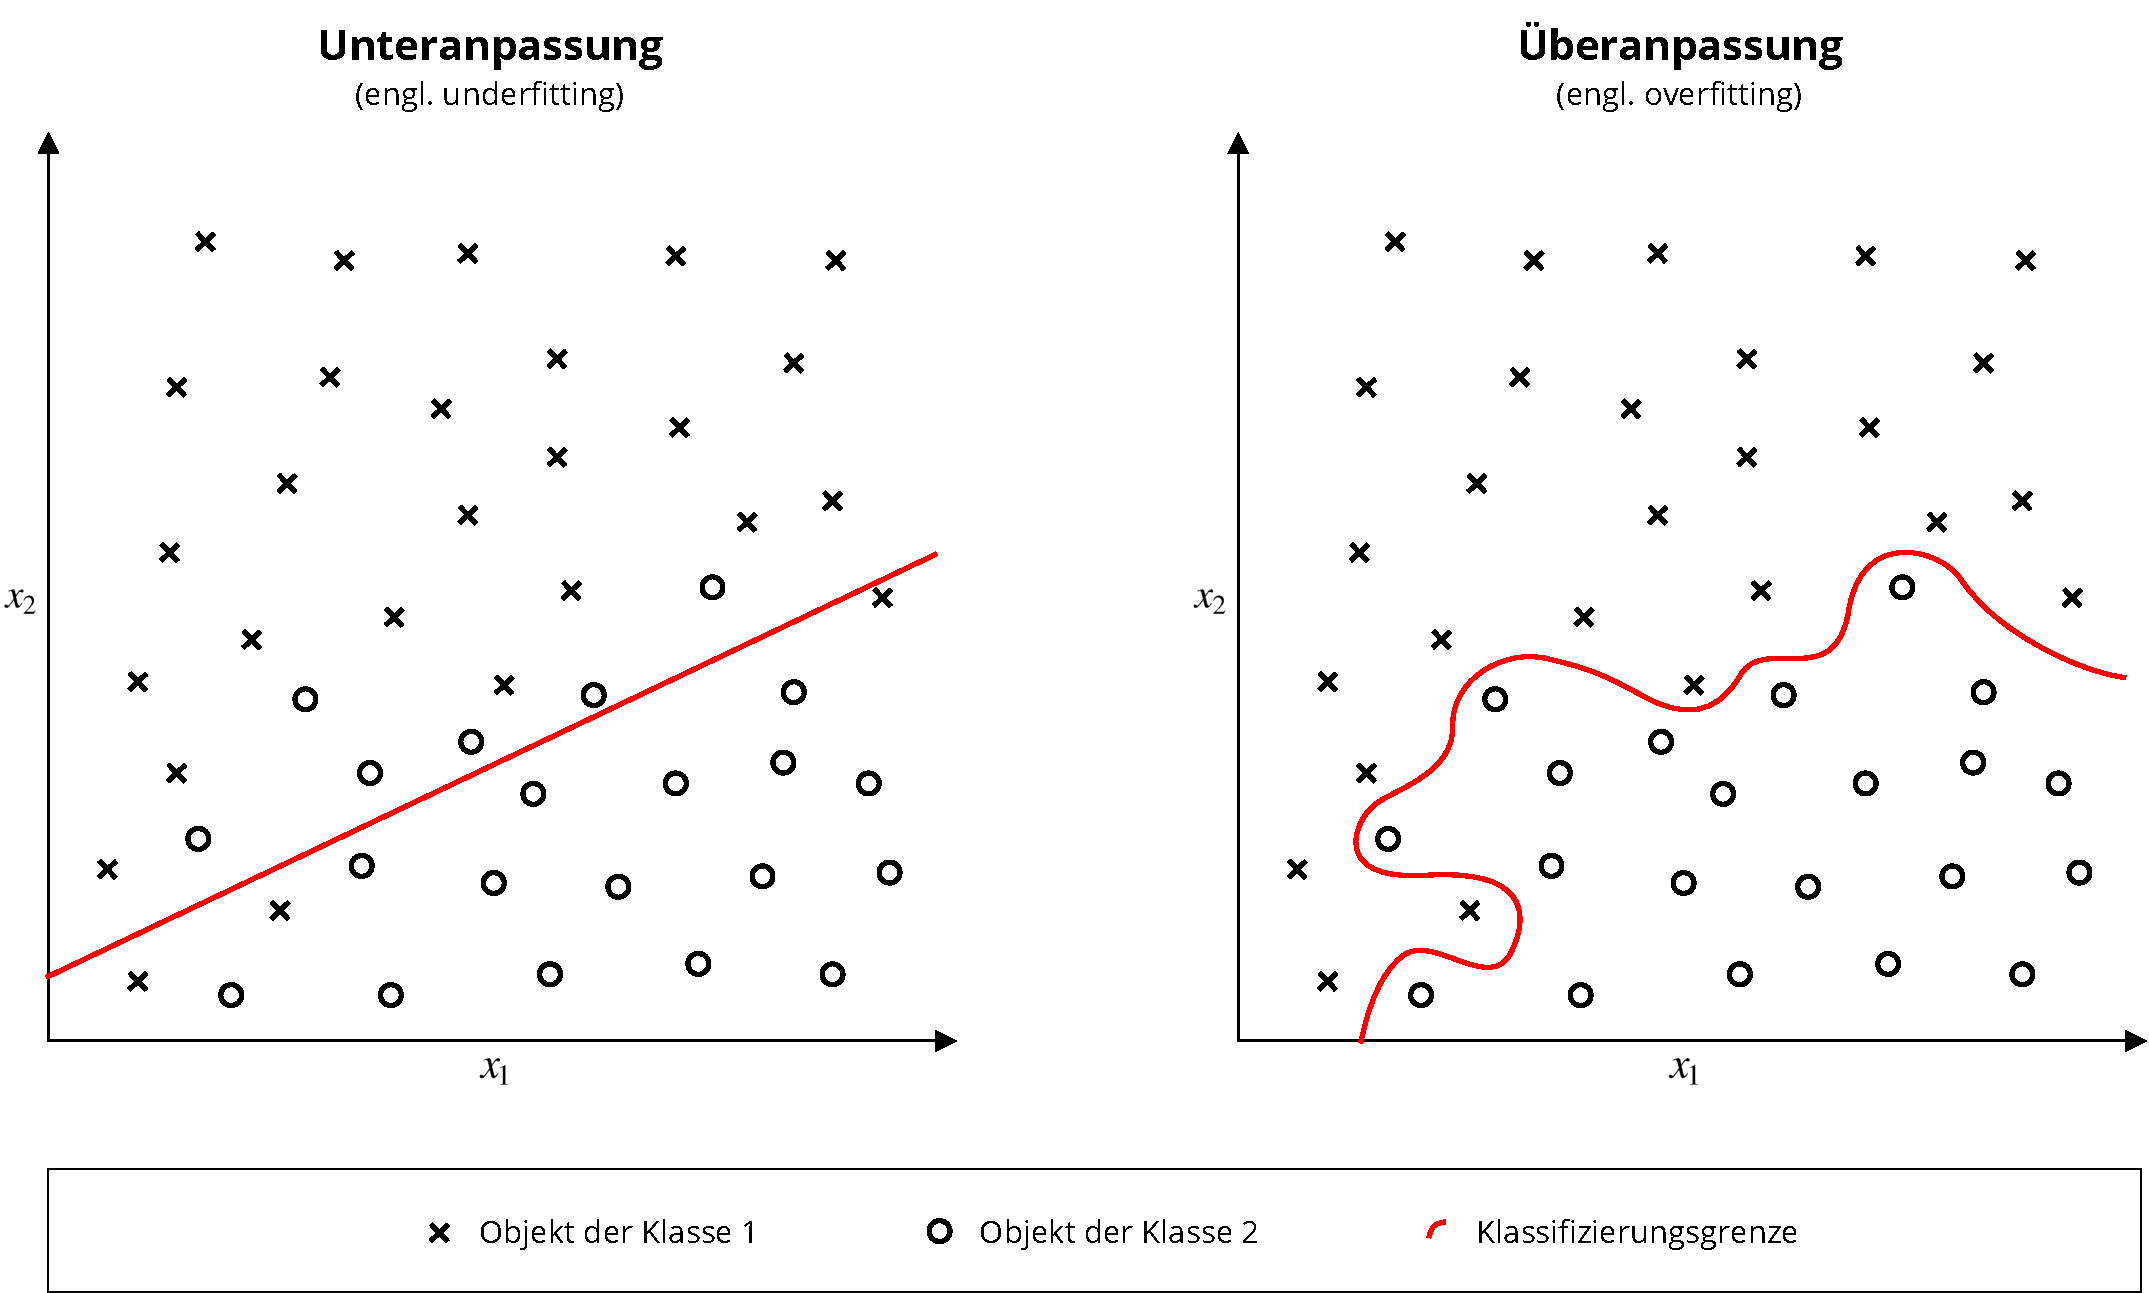
\includegraphics[scale=0.4]{overfitting.pdf}
\caption{Beispiel einer Unter- und Überanpassung bei einer Klassifizierung}
\label{fig_overfitting}
\end{figure}






% ===========================
\subsection{Entwicklung von künstlichen neuronalen Netzen}
\label{grundlagen_nn_entwicklung}
% ===========================

Duis autem vel eum iriure dolor in hendrerit in vulputate velit esse molestie consequat, vel illum dolore eu feugiat nulla facilisis at vero eros et accumsan et iusto odio dignissim qui blandit praesent luptatum zzril delenit augue duis dolore te feugait nulla facilisi.


\begin{equation}
a=b
\end{equation}

Definition DNNs


% ===========================
\subsection{Convolutional Neural Networks}
\label{grundlagen_nn_cnn}
% ===========================

Duis autem vel eum iriure dolor in hendrerit in vulputate velit esse molestie consequat, vel illum dolore eu feugiat nulla facilisis at vero eros et accumsan et iusto odio dignissim qui blandit praesent luptatum zzril delenit augue duis dolore te feugait nulla facilisi. 


% ===========================
\subsection{Recurrent Neural Networks und LSTMs}
\label{grundlagen_nn_rnn}
% ===========================

Lorem ipsum dolor sit amet, consectetuer adipiscing elit, sed diam nonummy nibh euismod tincidunt ut laoreet dolore magna aliquam erat volutpat. 


% ===========================
\subsection{Training mit synthetischen Daten}
\label{grundlagen_nn_synthetisch}
% ===========================

Lorem ipsum dolor sit amet, consectetuer adipiscing elit, sed diam nonummy nibh euismod tincidunt ut laoreet dolore magna aliquam erat volutpat. 


% ===========================
\subsection{Klassifizierung von Videos}
\label{grundlagen_nn_video}
% ===========================

Lorem ipsum dolor sit amet, consectetuer adipiscing elit, sed diam nonummy nibh euismod tincidunt ut laoreet dolore magna aliquam erat volutpat. 


